\documentclass{mpaper}

\begin{document}

\title{Measuring Software Ticket Quality using Statistical Analysis}
\author{Andrei-Mihai Nicolae}
\matricnum{2147392}

\maketitle

\begin{abstract}
Software tickets are of valuable importance to the whole computing science 
field - they guide engineers towards better planning, management 
and tracking of their progress throughout complex projects. However, there
are few studies that investigate what makes for a high quality,
valuable ticket. This can lead to multiple issues in a company, such as 
increased communication friction between developers and end users filing bug
reports, as well as increased overall costs due to waste of development effort. 
In this research paper, we present our findings after 
investigating a large number of variables surrounding software tickets, 
such as whether the presence of stack traces influence the time 
to close for the ticket. Our results show that the presence and type of attachments,
comments complexity (i.e. number of comments per ticket), grammar correctness scores
as well as the sentiment drawn from the comments can influence the quality of the ticket.
We bring a couple of novel aspects to the research
community including one of the largest dataset statistically analysed in the field,
as well as state-of-the-art sentiment and grammar correctness analysis.
\end{abstract}

\section{Introduction}

This paper outlines the standard template for an MSci submission.
In earlier years, MSci students at the School of Computing
Science,
University of Glasgow, were expected to produce a full-length
dissertation. Now, the requirement is for MSci students to
write a paper of up to 14 pages in length, using the supplied
\texttt{mpaper} \LaTeX style file.

The precise structure of an MSci paper is not mandated, but it should
probably cover in detail the following aspects of the project.
\begin{enumerate}
\item General description of the problem, motivation, relevance
\item Background information, possibly including a literature survey
\item Description of approach taken to solve the problem, including
  high-level design and lower-level implementation details as appropriate
\item Evaluation, qualitative or quantitative as appropriate
\item Conclusion, including scope for future work
\end{enumerate}

\section{Related Work}

This \LaTeX template is based on the ACM \texttt{sig-alternate} class.
The layout is two-column text. Generally figures and tables only
extend to one column width, e.g.\ Table \ref{tab-eg},
but it is possible to make them
stretch over both columns using the \texttt{figure*} and
\texttt{table*} environments. For an example, see Figure \ref{fig-eg}.

\begin{table}
\begin{tabular}{l||c||p{2cm}}
\emph{Operating System} & \emph{Version} & \emph{Verdict} \\ \hline \hline
Ubuntu & 12.04 & Everyone's favourite Linux, unless you grew up with
RedHat \\ \hline
Slackware & xxx & Pseudo-hacker's Linux, how often do you recompile
your kernel? \\ \hline
Mac OS & 10.7 & For people with more money than sense \\ \hline
\end{tabular}
\caption{\label{tab-eg}Single column table of figures}
\end{table}

\begin{figure*}
\begin{center}
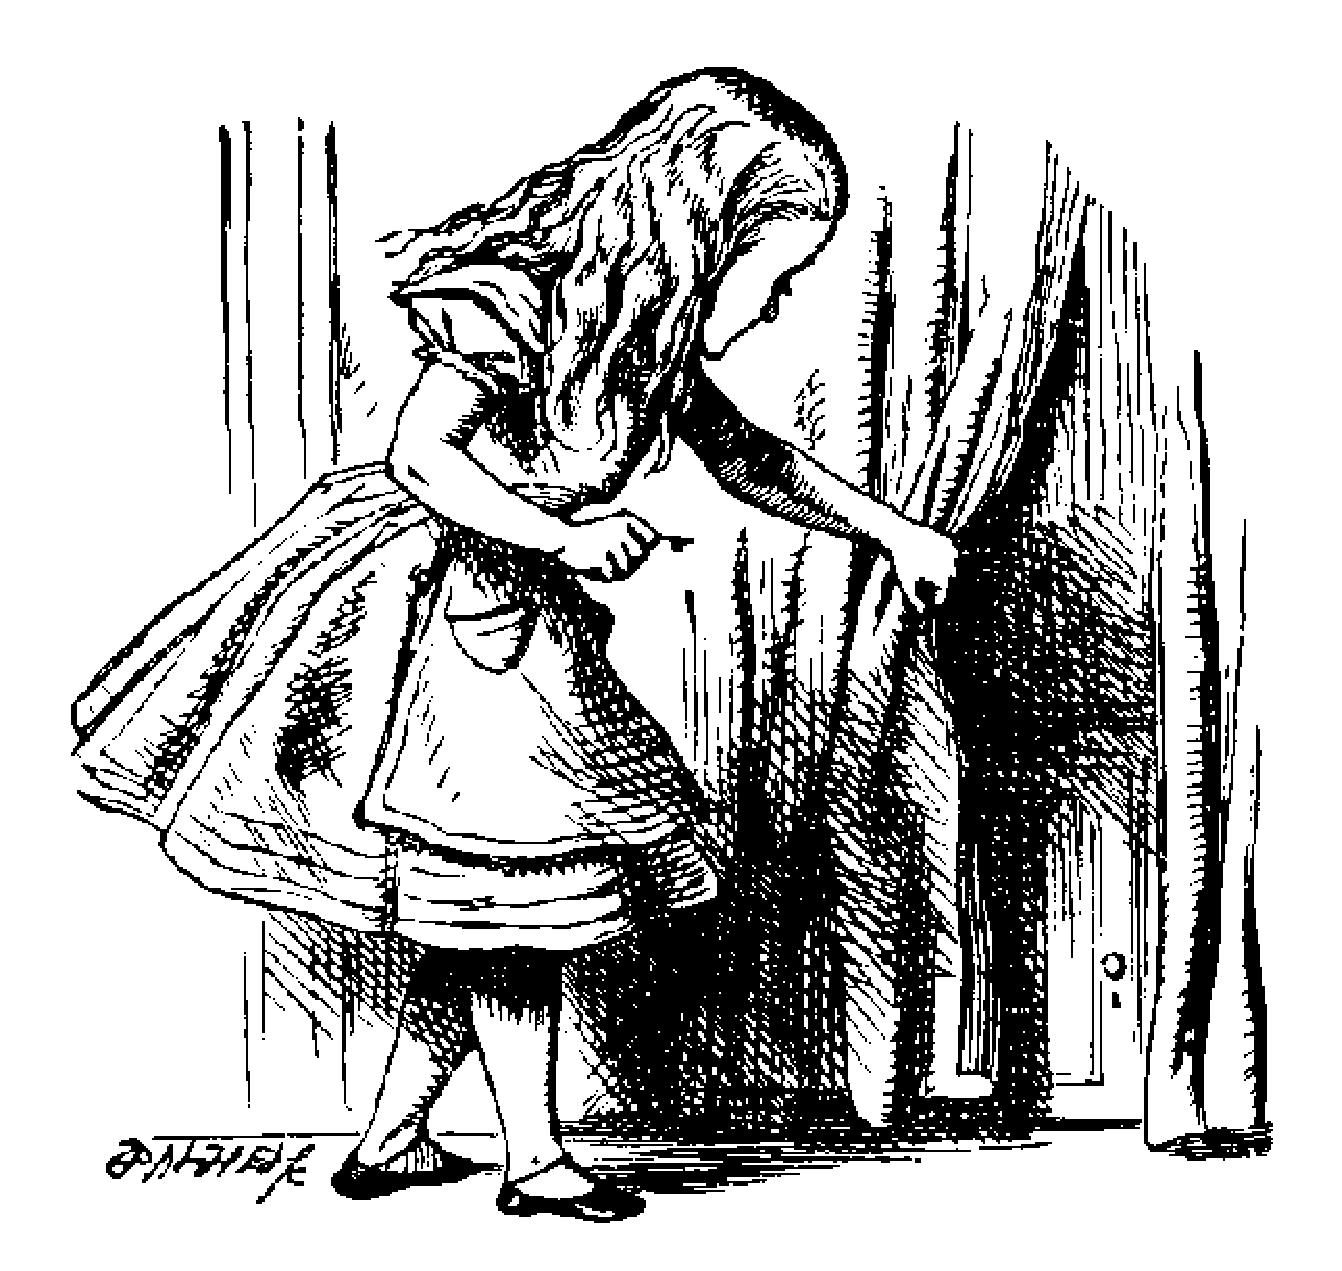
\includegraphics[scale=0.3]{images/alice.pdf}
\end{center}
\caption{\label{fig-eg}An example figure stretching over two columns}
\end{figure*}

\section{Building the Data Set}

Again, Simon Peyton Jones has a lovely description of how to write a
paper on his
website.
Personally, I put URLs in footnotes and \emph{bona fide} references
in the bibliography. For instance, Turing \cite{turing37computable}
and Knuth \cite{knuth68art} would not be out of place in list of
references.
How many references? Hard to say. Five is not enough, 50 is pushing
it.

\subsection{User Interface}

Blah blah blah
Blah blah blah
Blah blah blah
Blah blah blah

% - - - - - - - - - - - - - - - - - - - - - - - - - - - - - - - - - - - - - - -
\subsection{Foo}

Blah blah blah
Blah blah blah
Blah blah blah

\subsubsection{Bar}
\textsf{Blah} \textit{blah} \textbf{blah}

\section{Characterising the Data Set}

Graphs are always good. I recommend getting to grips with Matlab, R or
gnuplot rather than exporting horribly Excel bitmapped graphs.

\section{Correlations}

\section{Future Work}

\section{Conclusions}

\vskip8pt \noindent
{\bf Acknowledgments.}
Tim, my parents, Corina.

\bibliographystyle{abbrv}
\bibliography{paper}


\end{document}
